\documentclass{article}
\usepackage{amsmath,amssymb,amsthm,mdframed,kotex,paralist}
\usepackage{tabto}
%\TabPositions{0.5\textwidth}
\TabPositions{0.33\textwidth,0.66\textwidth}
\newcommand\bp[1]{\begin{mdframed}[frametitle={#1},skipabove=10pt,skipbelow=20pt,innertopmargin=5pt,innerbottommargin=40pt]}
\newcommand\ep{\end{mdframed}\par}
\newcommand\ov[1]{\ensuremath{\overline{#1}}}
\newcommand{\vs}{\vspace{0.05\textheight}}
\newcommand{\vvs}{\vspace{0.1\textheight}}
\newcommand{\vvvs}{\vspace{0.15\textheight}}

\begin{document}
\title{테스트 문제들}
\author{}
\date{\today}
\maketitle


\bp{01}
다음을 전개하여라.\par
(1) \((x+2)^2\)\par
(2) \((x-1)^3\)
\vs\ep

\bp{02}
다음 명제의 참 거짓을 판별하시오.\par
(1) 실수 \(x\), \(y\)에 대해 \(xy=0\)이면 \(x=0\) 또는 \(y=0\)이다.\par
(2) 실수 \(x\), \(y\)에 대해 \(x+y=5\)이면 \(x=2\)이고 \(y=3\)이다.\par
(3) 정수 \(m\)에 대해, \(m\)이 3의 배수이면 \(m^2\)도 3의 배수이다.\par
(4) 정수 \(m\)에 대해, \(m^2\)이 3의 배수이면 \(m\)도 3의 배수이다.
\vs\ep

\bp{03}
다음 일차함수에 대해 물음에 답하시오.
\[y=3x+6\]
(1) 이 함수의 그래프의 기울기를 구하시오.\\
(2) 이 함수의 그래프의 x절편을 구하시오.\\
(3) 이 함수의 그래프의 y절편을 구하시오.\\
(4) 이 함수의 그래프를 아래 모눈 위에 나타내시오.\\
(5) \(A=(3,a)\)가 그래프 위에 있을 때 \(a\)의 값을 구하시오.\\
(6) \(B=(b,27)\)가 그래프 위에 있을 때 \(b\)의 값을 구하시오.\\
(7) \(3x+6>0\)을 만족하는 \(x\)의 범위를 구하시오.\\
\vvs\ep
\begin{figure}[h!]
\centering
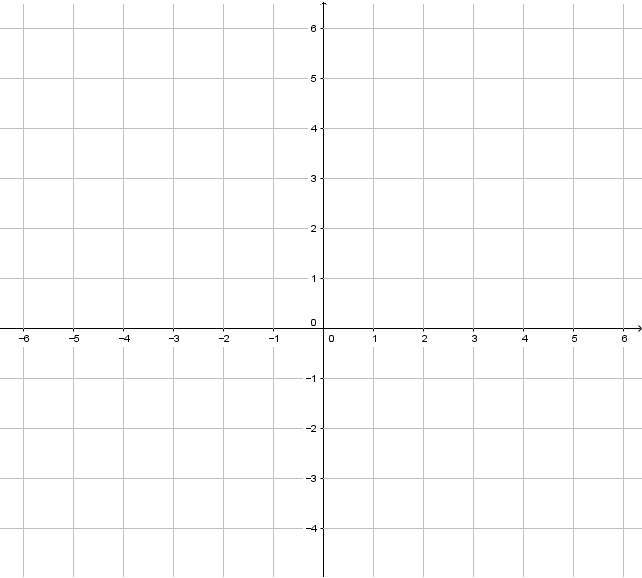
\includegraphics[width=.7\textwidth]{grid}
\end{figure}

\bp{04}
다음 이차함수에 대해 물음에 답하시오.
\[y=x^2-2x-3\]
(1) 이 함수의 그래프의 x절편을 구하시오.\\
(2) 이 함수의 그래프의 y절편을 구하시오.\\
(3) 이 함수의 그래프의 꼭지점의 좌표를 구하시오.\\
(4) 이 함수의 그래프를 아래 모눈 위에 나타내시오.\\
(5) \(A=(2,a)\)가 그래프 위에 있을 때 \(a\)의 값을 구하시오.\\
(6) \(B=(b,12)\)가 그래프 위에 있을 때 가능한 \(b\)의 값을 모두 구하시오.\\
(7) \(x^2-2x-3>-3\)을 만족하는 \(x\)의 범위를 구하시오.
\vvs\ep
\begin{figure}[h!]
\centering
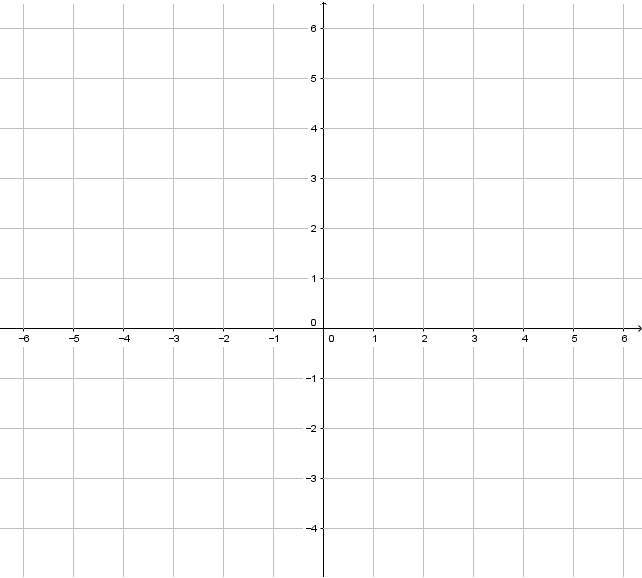
\includegraphics[width=.7\textwidth]{grid}
\end{figure}

\end{document}